\documentclass{article}
\usepackage{graphicx}
\usepackage[colorlinks=true,urlcolor=blue,linkcolor=cyan]{hyperref}
\title{How to run the abseir-family code}
\author{Gianfranco Giulioni}

\begin{document}
\maketitle


In this part of the manual we describe two ways of setting up for running simulations. The first one is the standard Repast procedure, where one can take advantage of various wizards to set up and run simulations. Although this provides several facilities, some user could feel uncomfortable with this standard process and would like to revert to a more basic procedure. The streamlined installation is for these users. It behooves to point out that the streamlined procedure was especially designed for running the model in the local machine and in batch mode. Therefore, the supporters of the Unix like command line interface will appreciate it. To help clarifying, it is worth to say that the streamlined procedure was developed to avoid the slowness of the wizards when continuously checking the effects of introducing new lines of code. It allows to run the model from the command line by typing two keys (i.e arrow up key - to recall the execution command, and the enter key). 


\section{Installation}

In this section we describe the standard installation process needed to prepare the system to run simulations. After taking the steps described below, the user should be able to run the model regardless of the operative system s/he is using.

The model needs Repast Symphony (RS), who in turn needs the Java Development Kit (JDK). Therefore we need first to check if the JDK is installed in the system and install it if needed. Once JDK is properly running, we have to install RS. Finally the model can be installed and run in RS.

\subsection{Java Development Kit (JDK)}

Check the list of installed software to know if JDK is installed in your system. If yes, note the JDK version.
Alternatively, you can open the command line interface of your system, type \verb+javac -version+ and hit the return key. 

Once verified if JDK is installed and, if yes, its version, visit the following URL:\\
\url{http://www.oracle.com/technetwork/java/javase/downloads/index.html}\\
to know which is latest released version of JDK.

If JDK is not installed in your system or if it is not at the latest release, follow the instruction found in the JDK download page to install or upgrade it. You can also search the internet for alternative ways to install or upgrade the JDK on your system.

This installation phase is complete when the \verb+javac -version+ command returns what you expect.
If not, you should fist check if the folder containing the JDK executables are in your execution path and add it manually if needed.
Furthermore, some Linux distribution must be informed on which JDK to use using the \verb+update-alternatives+ command. 

\subsection{Repast Simphony (RS)}

The Repast suite website: \url{http://repast.sourceforge.net} has all the information needed to download and install RS.

Note that RS is provided as a plugin of the eclipse Integrated Development Environment. The Repast development team provides a customized version of eclipse, so you could encounter problems with already installed versions of eclipse. Note that the streamlined installation provided below show how to avoid using eclipse.

\subsection{abseir\_family}

abseir\_family has to be installed as an eclipse RS project. We will give hereafter the instructions to achieve this goal.

First of all, open eclipse.

Suppose your workspace has the following path:\\
\verb+/Users/coolcoder/Documents/workspace+

Open the RS perspective (window $\rightarrow$ open perspective).

Create a new RS project called \verb+abseir_family+ (file $\rightarrow$ new $\rightarrow$ Repast Simphony project)

This creates the \verb+abseir_family+ folder and a series of sub folders inside the workspace:

The following figure show the \verb+abseir_family+ project folders tree.

\vskip2mm
\noindent
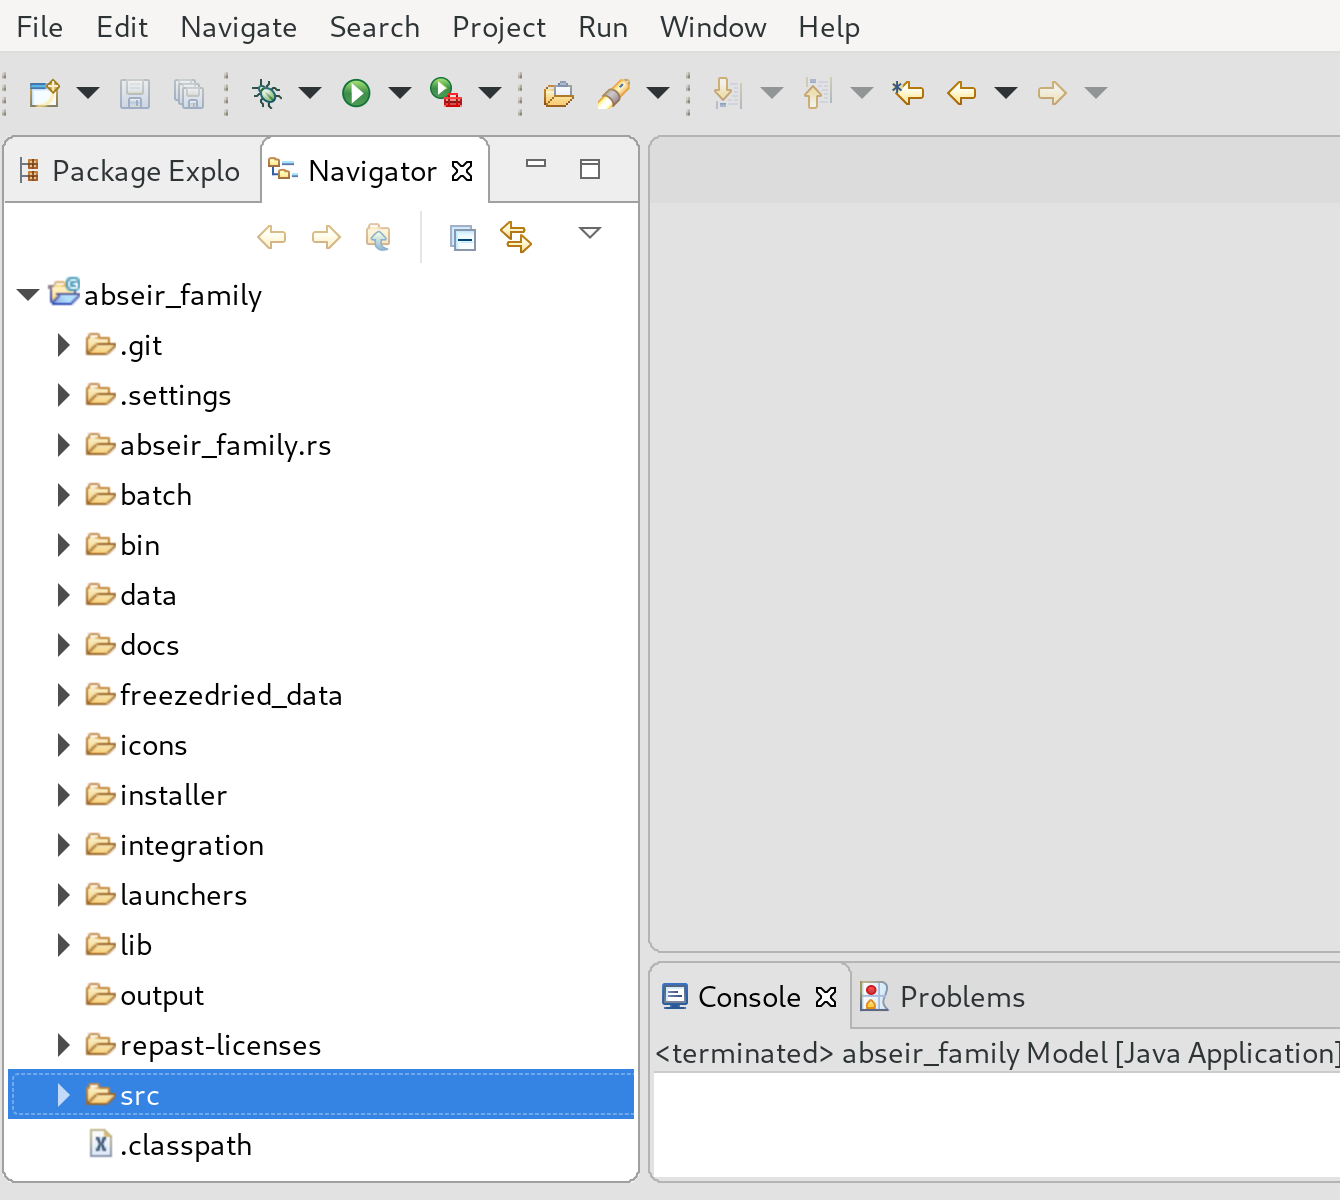
\includegraphics[scale=0.2]{fig_abseir_rs_navigation}


\vskip2mm
Now, the \verb+abseir_family+ files have to be added to the just created RS project folders tree.

We give here two alternatives: via git and using a zipped archive.

\subsubsection{Using git}

As you probably know, this is a popular way to share code. 
To fetch abseir\_family code, a git client need to be installed in your system. Many system comes with a git client already installed; if it is not your case, you have to install it. Mac and windows users can consider to install the GitHub Desktop software.

You can verify if git is installed in your system by checking if your command line interface recognize the \verb+git+ command.  
If your check is successful, change directory to the abseir\_family project folder:\\
\verb+cd /Users/coolcoder/Documents/workspace/abseir_family+\\
and type the following commands:
\begin{verbatim}
git init
git remote add origin https://github.com/gfgprojects/abseir_family.git
git fetch origin main
git reset --hard FETCH_HEAD
\end{verbatim}

Then if you plan to make your code changes available on GitHub, add the command:\\
\verb+git push --set-upstream origin main+

Now, the abseir\_family files should show up in the RS project folders.
Refresh the abseir\_family RS project with the navigation tab selected in the side bar (file $\rightarrow$ refresh) to make them visible in eclipse.

The following figure show how the \verb+src+ sub folder should look like.

\vskip2mm
\noindent
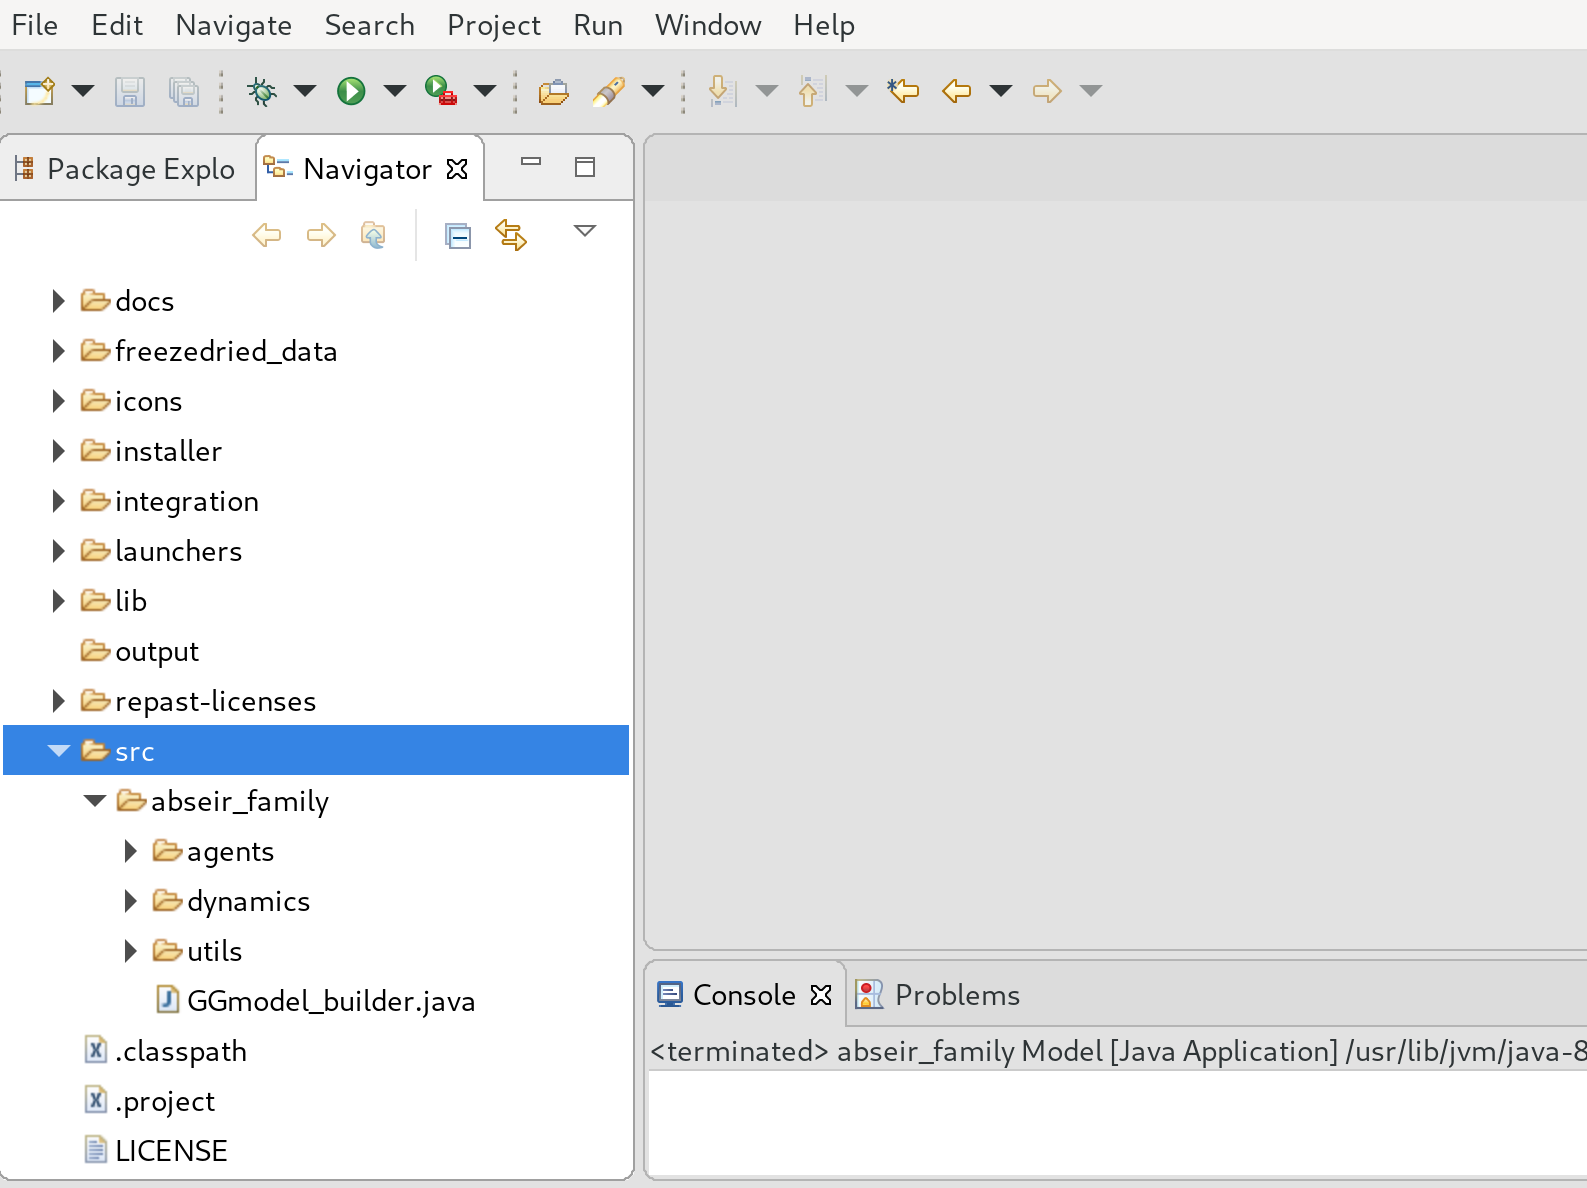
\includegraphics[scale=0.2]{fig_abseir_rs_navigation1}

\vskip2mm

\subsubsection{Using a zip archive}
Point your browser to\\ 
\verb+https://github.com/gfgprojects/abseir_family+\\
Click the ``code'' button and choose ``download zip''.

This will download the \verb+abseir_family-main.zip+ file in your system.

Unpacking it creates the abseir\_family-main folder.
Move the whole content of this folder in the abseir\_family RS project folder:\\  
\verb+/Users/coolcoder/Documents/workspace/abseir_family/+\\
Choose to overwrite existing files and folders if you will be asked (this will merge folders). 
Now refresh eclipse (file $\rightarrow$ refresh).



\section{Testing the Installation}


First you have to start the RS GUI window. To do so, click on the down black arrow highlighted by the red circle in the following picture

\noindent
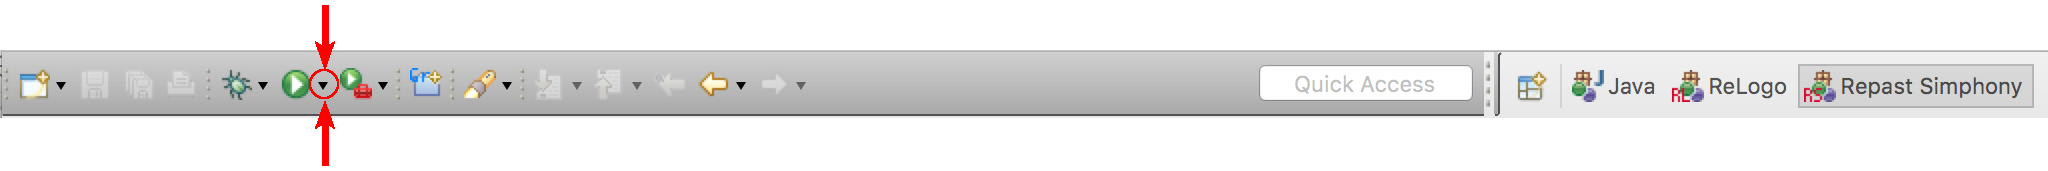
\includegraphics[scale=0.195]{fig_gabriele_rs_execution1a}

After clicking, a menu opens. Click the \verb+abseir_family Model+ item

After a while, the RS GUI (displayed in the following figure) will show up

\noindent
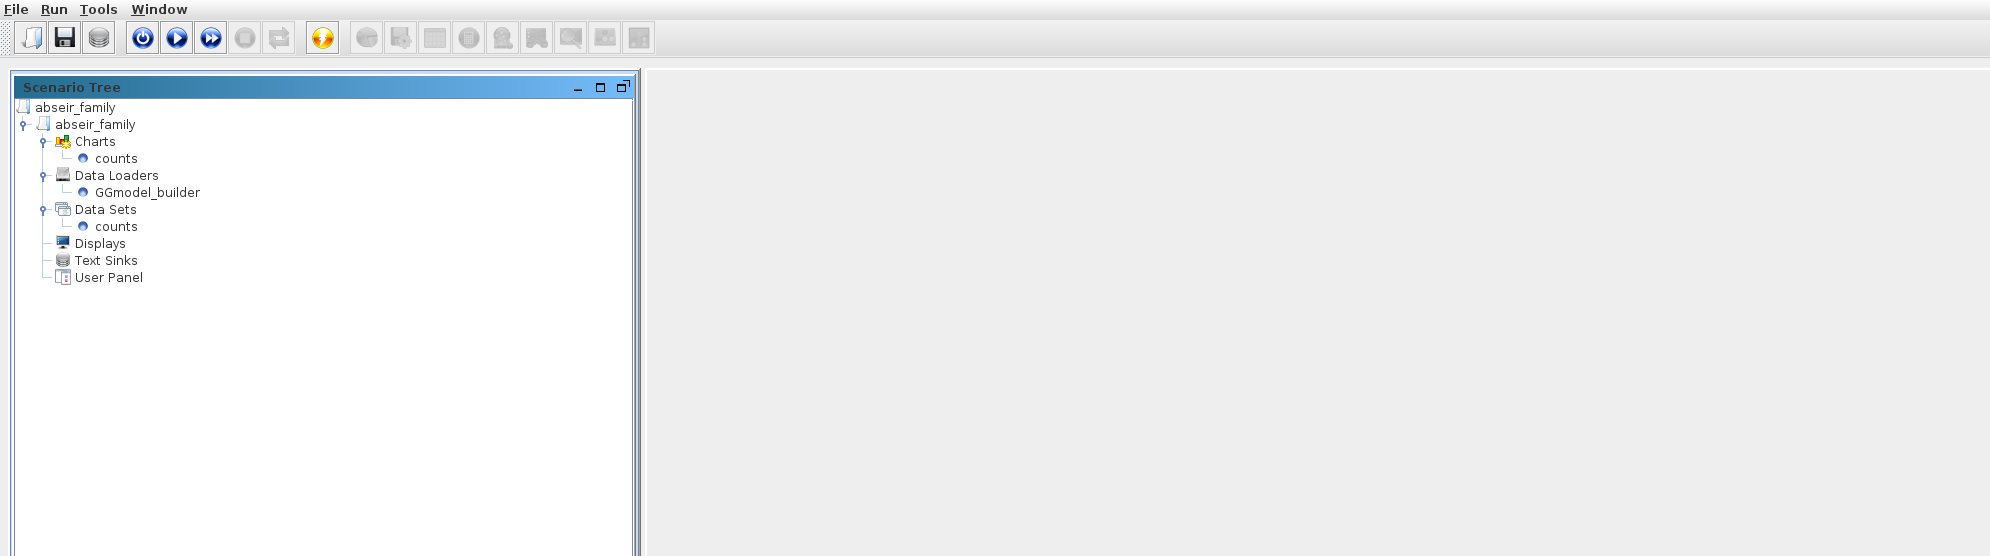
\includegraphics[scale=0.2]{fig_abseir_family_rs_gui0}

Check the \verb+Data Loaders+ item in the Scenario Tree. If the \verb+GGmodel_builder+ sub-item is reported (as in the screen shot above), the model can be run. Otherwise, contact \verb+gianfranco.giulioni@unich.it+. 

Now you can use the RS GUI window intuitive buttons to interact with the simulation. A more detailed description on how to control the simulation is given in the ``Repast Java Getting Started'' document available in RS web site.

The RS GUI window will look as in the figure below 

\noindent
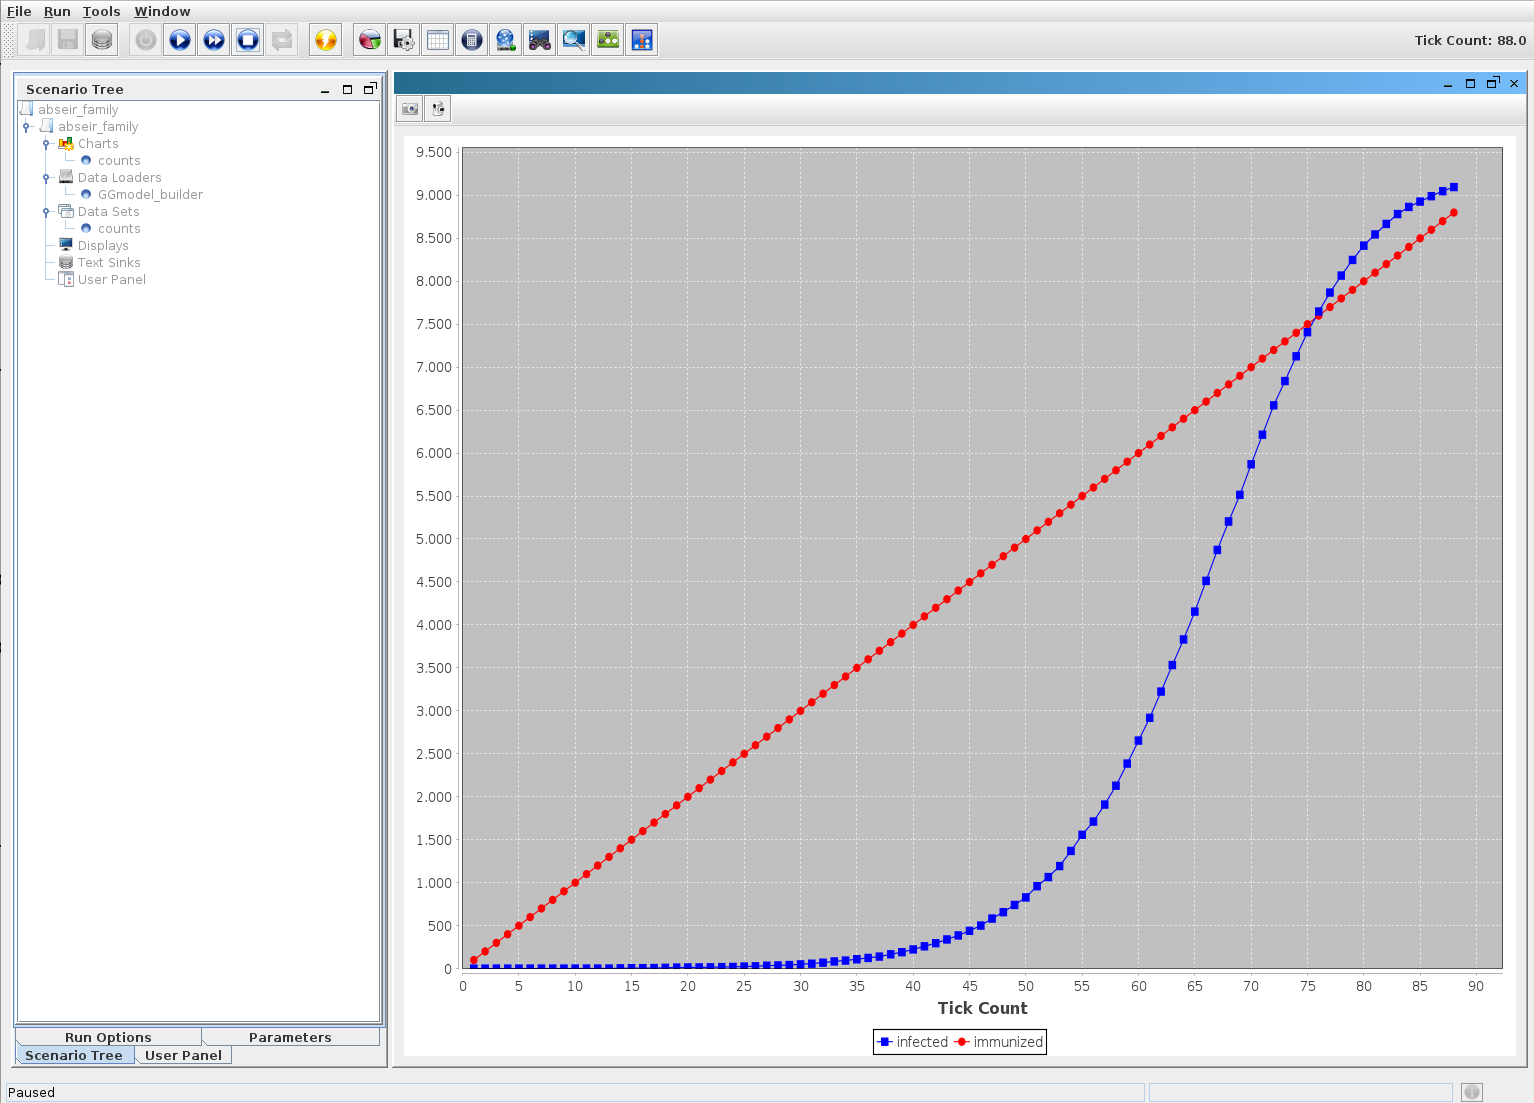
\includegraphics[scale=0.2]{fig_abseir_family_rs_gui1}



In addition to the just experienced GUI mode, the model can be run in BATCH mode. 

The GUI mode can be of great visual impact because several monitoring devices continuously updating during the run can be added to the RS GUI window. The flip side of the coin is that these devices slow down simulation execution. Second, the simulation runs exclusively in a machine running an X server. Notwithstanding the GUI mode can be a valid tool during the model development. When massive simulations are performed, the BATCH mode should be used instead. BATCH mode runs are faster because all the graphics elements are turned off. Furthermore, the absence of graphics makes it possible to run the model in parallel on several machines. It is worth saying that RS has very useful facilities for running a model in parallel.

\end{document}
